\documentclass[openany]{book}

\input{../../../latex_preambule_style/preambule}
\input{../../../latex_preambule_style/styleCoursLycee}
\input{../../../latex_preambule_style/styleExercices}
 \input{../../../latex_preambule_style/bas_de_page_cycle4}


%%%%%%%%%%%%%%%  Affichage ou impression  %%%%%%%%%%%%%%%%%%
\newcommand{\impress}[2]{
\ifthenelse{\equal{#1}{1}}  %   1 imprime / affiche sur livre  -----    0 affiche sur cahier 
{%condition vraieé
#2
}% fin condition vraie
{%condition fausse
}% fin condition fausse
} % fin de la procédure
%%%%%%%%%%%%%%%  Affichage ou impression  %%%%%%%%%%%%%%%%%%
 \usepackage{geometry}
 \geometry{top=2.5cm, bottom=0cm, left=2cm , right=2cm}
%%%%%%%%%%%%%%%%%%%%%%%%%%%%%%%%%%%%%%%%%%%%%%%%

\begin{document}


\begin{titre}[Les triangles]

\TitreSansTemps{Théorème de Thalès} 
\end{titre}


\begin{CpsCol}
\textbf{}
\begin{description}
\item[$\square$] Calculer une longueur dans un triangle
\end{description}
\end{CpsCol}




\begin{Th}
On considère :	
\begin{itemize}
\item un triangle ABC ; 
\item un point $M$ du segment $\left[AB\right]$, distinct de $A$ ;
\item un point $N$ du segment $\left[AC\right]$, distinct de $A$. 
\end{itemize}
Si les droites $\left(MN\right)$ et $\left(BC\right)$ sont parallèles	alors on a :$\frac{AM}{AB}=\frac{AN}{AC}=\frac{MN}{BC}$ .
\end{Th}





\begin{Rq} 
les dimensions du triangle $AMN$ sont proportionnelles aux dimensions du triangle $ABC$.
Le coefficient de proportionnalité est $\frac{AM}{AB}$ ou $\frac{AN}{AC}$ ou encore $\frac{MN}{BC}$.
\end{Rq}

\begin{Ex}

\begin{multicols}{2}
Sur la figure ci-contre :
$\left(YT\right)$ est parallèle à $\left(OJ\right)$ ;
$RT = 3$ cm ;
$RO = 5$ cm ;
$RY = 4,5$ cm.
Calculons $RJ$.
Je sais que :
\begin{itemize}
\item $ROJ$ est un triangle ;
\item $Y \in \left[RJ\right]$ ;
\item $T \in \left[RO\right]$ ;
\item $\left(YT\right)$ est parallèle à $\left(OJ\right)$
\end{itemize}
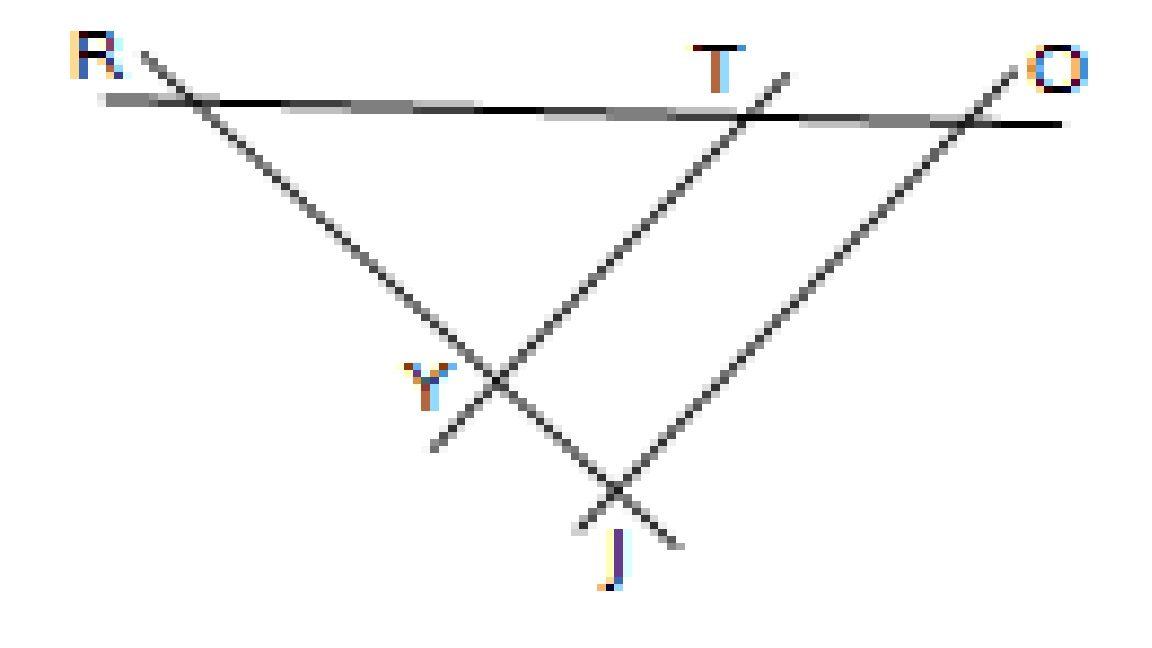
\includegraphics[scale=0.3]{cours1.jpg}  
\end{multicols}


Donc, d'après le théorème de Thalès, je peux dire que : $\frac{RY}{RJ}=\frac{RT}{RO}=\frac{YT}{JO}$ (on écrit l'égalité des trois quotients).
\\Donc $\frac{4,5}{RJ}=\frac{3}{5}=\frac{YT}{JO}$ (on remplace les longueurs connues par leurs valeurs).
\\Comme $\frac{4,5}{RJ}=\frac{3}{5}$ (on ne conserve qu'une seule égalité), on déduit que $4,5 \times 5=3\times RJ$ (on écrit l'égalité des \og produits en croix \fg{}.
\\Finalement $RJ= \frac{4,5 \times 5}{3}$  (on \og isole \fg{} la longueur cherchée) et donc $RJ=7,5$ cm (on conclut).
\end{Ex}


Exercices sur le livre :

\begin{description}
\item[12 et 14 p 252] Représenter. Communiquer.
\item[17 p 252] Calculer. Communiquer.
\item[45 p 257] Représenter. Communiquer.
\item[19 p 252 à la maison] Représenter. Communiquer.
\item[49 p 258 à la maison] Calculer. Communiquer.
\item[50 p 259] Calculer. Communiquer.
\end{description}


\subsection{Agrandissement et Réduction}

\begin{Def}
Si	deux figures ont la même forme et des longueurs proportionnelles, 
alors	on dit que l'une est un \textbf{agrandissement ou une réduction} de l'autre.
\end{Def}

\begin{Rq}
Le coefficient de proportionnalité est le rapport d'agrandissement ou de réduction.
\end{Rq}

\begin{Ex}
\begin{multicols}{2}
$DEF$ est un agrandissement de $ABC$ de rapport $1,6$. Calculons les longueurs de ses côtés.
\\$DE = 1,6 \times AB = 1,6 \times 1,5 = 2,4$ cm
\\$DF = 1,6 \times AC = 1,6 \times 2,5 = 4$ cm
\\$EF = 1,6 \times BC = 1,6 \times 3,2 = 5,12$ cm
\\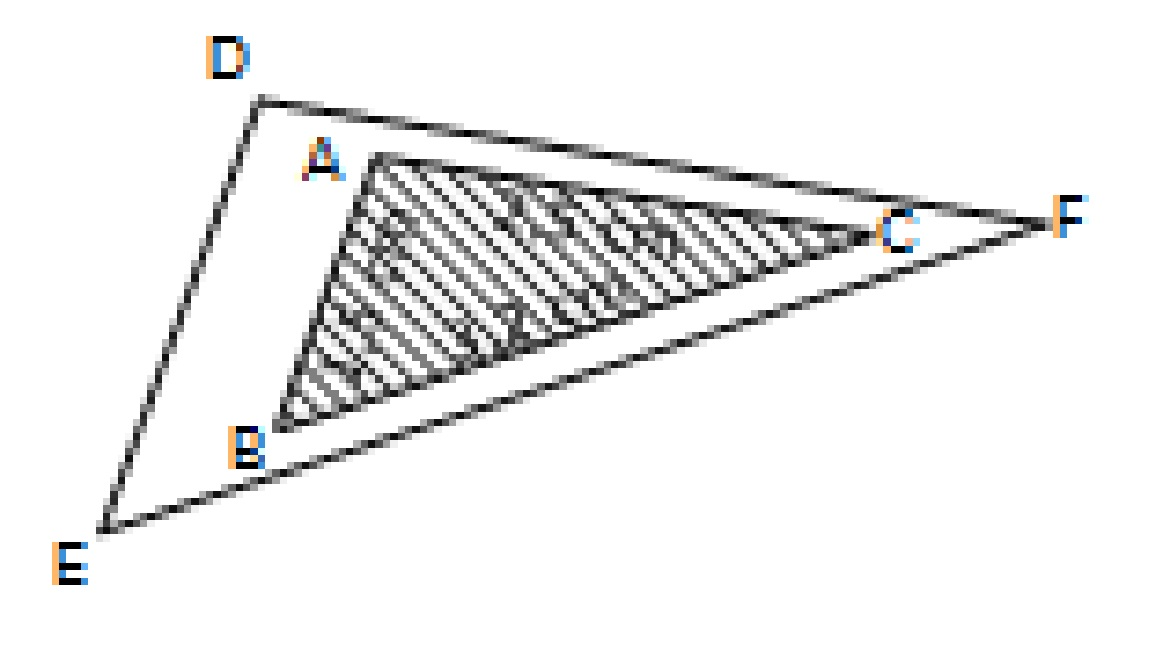
\includegraphics[scale=0.25]{cours2.jpg}  
\end{multicols}
\end{Ex}

\begin{Rq} 
\begin{itemize}
\item $ABC$ est une réduction de $DEF$ de rapport $\frac{1,5}{2,4}  = \frac{2,5}{4} =\frac{3,2}{5,12}  = 0,625$.
\item Dans un agrandissement ou une réduction, les mesures des angles, la perpendicularité 
et le parallélisme sont conservés.
\end{itemize}
\end{Rq}








\end{document}